\documentclass[10pt]{article}
%\documentclass[review]{siamart1116}
%\documentclass[review]{siamonline1116}

\usepackage{amsmath}
\usepackage{amsfonts}
\usepackage{amssymb}
\usepackage{fancyhdr}
\usepackage[margin=0.75in]{geometry}
\usepackage{graphicx}
\usepackage[section]{placeins}
\usepackage{nicefrac}
\usepackage{bm}
\usepackage{xcolor}
\usepackage[format=plain,indention=.5cm, font={it,small},labelfont=bf]{caption}
\usepackage{subcaption}
\usepackage{float}
\usepackage{enumerate}
\usepackage{tikz}
\usepackage[all]{xy}
\usepackage{url}



%%%%%%%%%%%%%%%%%%%%%%%%%%%%%%%%%%%%%%%%%%%%%%%%%%%%%%%%%%%%%%%%%%%%%%%%%%%%%%%%%%%%%%%%%%%%%%%%%%%%%%%%%%%%%%%%%%
\usepackage{stackengine}
\usepackage{amsthm}
\usepackage{cleveref}


\newtheorem{theorem}{Theorem}
\newtheorem*{theorem*}{Theorem}
\newtheorem{lemma}{Lemma}
\newtheorem*{lemma*}{Lemma}
\newtheorem*{conj}{Conjecture}
\newtheorem{corollary}{Corollary}
\newtheorem{clm}{Claim}
\newtheorem{rmk}{Remark}
\newtheorem{note}{NOTE}

\theoremstyle{definition}
\newtheorem*{def*}{Definition}
\newtheorem{definition}{Definition}
\numberwithin{theorem}{section}
\numberwithin{definition}{section}
\numberwithin{lemma}{section}
\numberwithin{corollary}{section}
\numberwithin{clm}{section}
\numberwithin{rmk}{section}

\newcommand{\low}[1]{$_{\text{#1}}$}
\newcommand\xput[2][0.5]{%
	\rule{#1\linewidth}{0pt}\makebox[0pt][c]{#2}\hfill}

\setlength{\headheight}{15pt}
\pagestyle{fancy}
\renewcommand{\headrulewidth}{0pt}
\fancyhead[L]{Brunner}
\fancyhead[C]{Co-Occurrance Network}
\fancyhead[R]{\today}
\lfoot{}
\cfoot{\thepage}
\rfoot{}

%%%%%%%%%%%%%%%%%%%%%%%%%%%%%%%%%%%%%%%%%%%%%%%%%%%%%%%%%%%%%%%%%%%%%%%%%%%%%%%%%%%%%%%%%%%%%%%%%%%%%%%%%%%%%%%%%%
%
%
%\newsiamthm{clm}{Claim}
%\newsiamremark{rmk}{Remark}
%\newsiamremark{note}{NOTE}
%\numberwithin{theorem}{section}
%
%
%%%%%%%%%%%%%%%%%%%%%%%%%%%%%%%%%%%%%%%%%%%%%%%%%%%%%%%%%%%%%%%%%%%%%%%%%%%%%%%%%%%%%%%%%%%%%%%%%%%%%%%%%%%%%%%%%%
\newenvironment{inbox}[1]
{\begin{center}
		\begin{tabular}{|p{0.9\textwidth}|}
			\hline\\
			{\bf #1}\\
		}
		{ 
			\\\\\hline
		\end{tabular} 
	\end{center}
}

\newcommand{\nhalf}{\nicefrac{1}{2}}
\newcommand{\eps}{\epsilon_{machine}}
\newcommand{\ol}{\overline}
\renewcommand{\b}{\bm}

\definecolor{dgreen}{RGB}{49,128,23}
\definecolor{nicepink}{RGB}{255, 0, 102}
\definecolor{nicered}{RGB}{255, 80, 80}

\newcommand{\bE}{\mathbb{E}}
\newcommand{\bP}{\mathbb{P}}
\newcommand{\bR}{\mathbb{R}}
\newcommand{\bN}{\mathbb{N}}
\newcommand{\bZ}{\mathbb{Z}}
\newcommand{\bQ}{\mathbb{Q}}
\newcommand{\bC}{\mathbb{C}}
\newcommand{\cA}{\mathcal{A}}
\newcommand{\cB}{\mathcal{B}}
\newcommand{\cC}{\mathcal{C}}
\newcommand{\cD}{\mathcal{D}}
\newcommand{\cE}{\mathcal{E}}
\newcommand{\cF}{\mathcal{F}}
\newcommand{\cG}{\mathcal{G}}
\newcommand{\cH}{\mathcal{H}}
\newcommand{\cI}{\mathcal{I}}
\newcommand{\cJ}{\mathcal{J}}
\newcommand{\cK}{\mathcal{K}}
\newcommand{\cL}{\mathcal{L}}
\newcommand{\cM}{\mathcal{M}}
\newcommand{\cN}{\mathcal{N}}
\newcommand{\cO}{\mathcal{O}}
\newcommand{\cP}{\mathcal{P}}
\newcommand{\cQ}{\mathcal{Q}}
\newcommand{\cR}{\mathcal{R}}
\newcommand{\cS}{\mathcal{S}}
\newcommand{\cT}{\mathcal{T}}
\newcommand{\cU}{\mathcal{U}}
\newcommand{\cV}{\mathcal{V}}
\newcommand{\cW}{\mathcal{W}}
\newcommand{\cX}{\mathcal{X}}
\newcommand{\cY}{\mathcal{Y}}
\newcommand{\cZ}{\mathcal{Z}}

\newcommand{\inter}{\text{\normalfont int}}
\newcommand{\ka}{\kappa}
\newcommand{\fp}{\varrho}
\newcommand{\problem}[2]{ \ \\ {\bf #1} {\it #2} \ \\} 

\renewcommand{\arraystretch}{1.5}
\renewcommand{\thefootnote}{\fnsymbol{footnote}}	
\author{Jim Brunner}
\title{Using a co-occurrance network}

\begin{document}
\maketitle
\section{Network Building}
We are looking at creating ecological networks of a microbiome. Right now, I have built two networks, in the form of graphs $\cG_1 = (\cV_1, \cE_1)$ and $\cG_2 = (\cV_2,\cE_2)$. In both graphs, vertex are labeled by taxa name. I'm going to conflate the vertices and their label. The edge sets are defined by co-incidence and co-occurence, respectively. Given a set of samples with abundancs of organisms, we map the abundances to discrete levels, as proportions of the maximum abundance \emph{of that organism}. Precisely, let the samples be $s_i$ and raw abundance of organism $j$ in sample $i$ be $r_{ji}$. I map the abundances according to
\[
a(r_{ji})  = \left\{
\begin{array}{c c}
\lfloor\left(\frac{r_{ji}}{\max_{s_k}(r_{jk})}\right) n \rfloor + 1 &  \frac{r_{ji}}{\max_{s_k}(r_{jk})} \geq m \\
0 & \frac{r_{ji}}{\max_{s_k}(r_{jk})} < m
\end{array}
\right.
\]
where $m$ is some minimum. Then, I create weighted edges between vertices (where $0$ weight means no edge exists) where the weights of edges in $\cE_1$ are
\[
w^1_{jk} = \frac{\|\{i: a(r_{ji}) = a(r_{ki}) \neq 0\} \|}{S}
\]
where $S$ is the total number of samples. That is, we count the propotion of samples in which the two taxa appear at the same discritized level. 

The second network accounts for random coincidence of taxa in a sample, following \cite{coocc}. It begins with $\cG_1$, and compares to a null model $N$. The null model is defined in the following way.
\[
A_j= \sum_{s_i} \b{1}_{a(r_{ji}) \neq 0}
\] 
and 
\[
S_i^l  = \sum_{v_j} \b{1}_{a(r_{ji}) = l}
\]
Then, $N$ assumes that if
\[
X_{jil} \sim \mathit{binom}\left(A_j, \frac{S_i^l}{\sum_{il} S_i^l}\right)
\]
then $P(a_{ji}^N = l) = 1-P(X_{jil} = 0)$. This allows us to calculate the probability of co-incidence of taxa under the null model. Let $w_{jk}^N$ be
\[
w^N_{jk} = \|\{i: a_{ji}^N = a_{ki}^N \neq 0\} \|
\]
This is the similar to the co-incidence model but now randomized. Then,
\[
P(w_{jk}^N = K) =  \sum_{\{A \subset \cV_2:|A| = k\}} \prod_{l\in A} a_{jl}a_{kl}\prod_{l \not\in A} (1- a_{jl}a_{kl})
\]
Ideally, we would then define $\cE_2$ by the weights
\[
w_{jk}^2 = \left\{ \begin{array}{c c}
1 & P(w_{jk}^N \geq w_{jk}^1) \leq t\\
0 & P(w_{jk}^N < w_{jk}^1) > t
\end{array}\right.
\]
However, that probability is intractible to compute. Instead, we take 
\[
\widetilde{P}(w_{jk}^N = K) = \sum_{l=0}^i \binom{N_1}{l}\binom{N_2}{K-l} p_1^j p_2^{K-l} (1-p_1)^{N-l}(1-p_2)^{N-K+l}
\]
where
\[
p_1 = p_a - \left(\frac{N_2}{N_1}\frac{N(\mu-\sigma^2)- \mu^2}{N^2}\right)^{\nhalf}
\]
and 
\[
p_2 = p_a - \left(\frac{N_1}{N_2}\frac{N(\mu-\sigma^2)- \mu^2}{N^2}\right)^{\nhalf}
\]
Finally, $N_1$, $N_2$ are to ensure that $p_1,p_2 \in [0,1]$. It turns out we need:
\[
\frac{\mu N (1-p_a) - N\sigma^2}{N(1-p_a)- \sigma^2} \leq N_2 \leq \frac{\mu^2}{\mu- \sigma^2}
\]
with $\mu$ the mean of the real distrubution, $\sigma^2$ the variance, and $p_a = \frac{1}{S}\sum_{i} a_{ji}a_{ki}$. So, we take 
\[
w_{jk}^2 = \left\{ \begin{array}{c c}
1 & \widetilde{P}(w_{jk}^N \geq w_{jk}^1) \geq t\\
0 & \widetilde{P}(w_{jk}^N < w_{jk}^1) > t
\end{array}\right.
\]

\section{Network Analysis}
We can cluster - community clustering, spectral clustering, comparing to random graphs. Comparison of clusters to grouping by sample type.

\section{Using the network to analyze a sample}

The question now is what can we do these networks?

First, assesing GOTTCHA reads. A single GOTTCHA read would produce a network with each connected component complete. I think the co-incidence network is more appropriate. We want to assess the probability that you see this set together. We have the probability that you see any vertex pair (estimated) as the edge weights of $\cG_1$. Precisely, the edge weights are
\[
w^1_{jk} = P(j \, \&\, k \in  S_i^l)
\]
where $S_i^l$ is sample $i$ at discrete abundance level $l$. It might be useful to have the directed weight graph where
\[
w^3_{jk} = P(j \in S_i^l | k \in S_i^l)
\]
but that wouldn't be hard, because then
\[
w^3_{jk} = S\frac{w^1_{jk}}{\|\{i:a(r_{ki})>0\}\|} 
\]
Anyway, let's start with the simplest case of one abundance level. Assume GOTTCHA found taxa $a,b,c,...,n$. Maybe the first thing we would want is
\[
P(a | b,c,d,...,n), \, P(b|a,c,d,...,n) ,\, \mathit{etc}
\]
Clearly, we can see directly $P(a|b)$, etc. We can also get a bound for triplets (assuming $P(c,b) \neq 0$):
\[
P(a|b,c) \leq \frac{\min_{(i,j) \subset \{a,b,c\}}(P(i,j))}{P(b,c)}
\]
but we can't do any better than triplets explicitly, because we don't have any sort of independence (conditional or otherwise) and because our network is not acyclic. 

We can probably learn something from asking about the connectivity of the induced subgraph. Notice that if it isn't complete, then one of the $P(a,b)$ is $0$ above. 

What does the connectivity of the induced subgraph of $\cG_2$ tell us? If it is connected, that's good.  We could use that network to identify vertices that are connected to many of the vertices in the induced subgraph - this might indicate that node should be in the sample.

I guess $\cG_2$ is a markov random field \cite{machine_learning}. This might give us a way to calculate the probability you see a group taxa (and maybe others). The main idea of a MRF is that nodes are conditionally independent of nodes they aren't neighbors of (conditioned on ones they are neighbors of). If $c$ are the (maximal) cliques of the graph (complete subgraphs), then the probability of configuration $\b{x}$ is
\[
P(\b{x}) = \frac{1}{Z} \prod_{c} \psi_c (x_{c})
\]	
where $Z$ is a normalizing constant and $\psi_c$ are potential functions I don't know how to come up with yet. Anyway, if we have a sample that contains (maybe as a subset) $s$, we can calculate something. Let $C_s$ be the cliques represented in $s$.
\[
P(\b{s}) = \frac{1}{Z}\sum_{\{\b{x} : s\subset \b{x}\}}\prod_{c\in C_s}\psi_c(\b{x})
\]
And we can ignore cliques not represented in $s$. We probably have to change $Z$. I guess we can also use neighbor pairs instead of maximal cliques. Either way we have to figure out what $\psi_c$ are.

\subsection{Determining $\psi_c$}

Before figuring out $\psi_c$, it should be noted that we have a choice of configuration space of the network. We can use a binary $\{1,0\}^N$ space to denote presence or absence, or we can choose a continuous space to include abundances. To begin, I will only consider presence \& absence.
	
\begin{inbox}{Snowshoe hairs and Canadian Lynx, CRNT}
Now I'm very tempted to think about how this approach relates to mass action dynamical systems. I'm going to think about my very favorite model.
\[
\b{\dot{x}} = \ka_1 x \begin{pmatrix} 1 \\ 0 \end{pmatrix} + \ka_2 xy \begin{pmatrix}
-1 \\ 1
\end{pmatrix} + \ka_3 y \begin{pmatrix}
0\\-1
\end{pmatrix}
\]
Well. Yes. But there is only one maximal clique so $P(\b{x}) = \psi (\b{x})$ and that's just whatever it is. We know that it evolves according to the stochastic mass action equations. In fact, the result that the stationary distribution is a product of poissons for a complex balanced system can be thought of as fitting into this framework. I wonder if you could use this theory to re-prove that? Recall that the stationary distribution for a complex balanced system with equilibrium $\b{c}$ is 
\[
\pi(\b{x}) = \frac{1}{Z} \prod_{i=1}^d \frac{c_i^{x_i}}{x_i!}
\]
so here we have that
\[
\psi_c = \prod_{i \in c} \frac{c_i^{x_i}}{x_i!}
\]
or taking cliques to be just singletons
\[
\psi_i = \frac{c_i^{x_i}}{x_i !}
\]	
I can't think of any way to arrive upon that directly, and so prove the result from this direction. Also, This is even more general than a MRF, as it has self-loops. Self loops play the role of time update. In fact, one might say that a MC is to a MRF as an ODE is to a PDE. Then, self loops in the MRF correspond to time derivatives or forcing appearing in the PDE.
\end{inbox}

It seems reasonable to use a pairwise RMF. It also seems reasonable to take a log linear function. My initial guess is
\[
\psi_{s\sim t} (y_s,y_t) = \exp(\b{\theta} \cdot \b{1}_{y_s = i,y_t = j})
\]
where $\theta = (0,\log(P(s)), \log(P(t)),\log(\nhalf(P(s|t) + P(t|s))))$. But that's a guess. It makes sense we have only unconnected nodes. It also also penalizes leaving out nodes that are connected to the nodes we do have. However, this penalizes us too harshly if we include a hub node.

Let's play with a small network to try to get a handle on this. Consider the network shown in \cref{toy_network}
\begin{figure}
	\begin{center}
	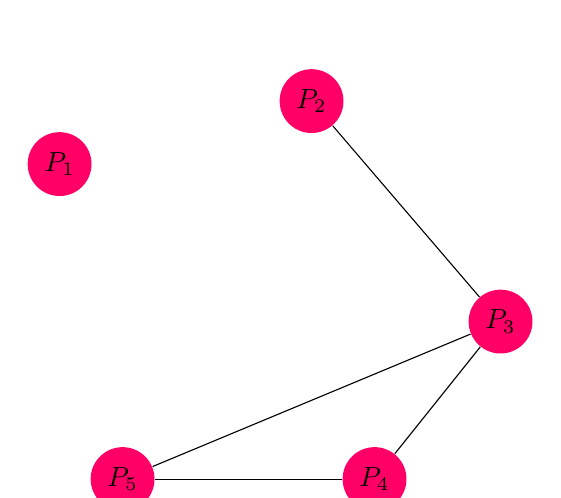
\begin{tikzpicture}[scale = 4]
	\node (a) at (0,1) [circle, fill = nicepink] {$P_1$};
	\node (b) at (0.8,1.2) [circle, fill = nicepink] {$P_2$};
	\node (c) at (1.4,0.5) [circle, fill = nicepink] {$P_3$};
	\node (d) at (1,0) [circle, fill = nicepink] {$P_4$};
	\node (e) at (0.2,0) [circle, fill = nicepink] {$P_5$};
	\draw (b) edge (c);
	\draw (c) edge (d);
	\draw (c) edge (e);
	\draw (d) edge (e);
	\end{tikzpicture}
	\end{center}
	\caption{A small network example}\label{toy_network}
\end{figure}
	
	
	
	
	
	
\bibliographystyle{plain}
\bibliography{../../summer17}
\end{document}